You can find the code and everything else also on GitHub under the link \textit{https://github.com/awilsee/CSec}. Maybe more convenient for you.


\section{Exploring Certificate Authority Public Key Infrastructure (CA-PKI) with OpenSSL}

\subsection{A}

Beside your descriptions I also have to change the following two options to get the web server in chapter \ref{t2} running. Additionally I have generated the ca-key with 2048 bits.

\begin{lstlisting}
default_bits		= 1024
CipherString = DEFAULT@SECLEVEL=1
\end{lstlisting}

\subsection{B}

\textit{What do you observe? What fields are there?} \\
It shows the data of the certificate with all the inputs from before. Additionally you can see that \textit{sha256WithRSAEncryption} is used for encryption. Further more the RSA public key is included.\\

\subsection{C}

\textit{Open the key file your just created with a text editor and note your observations.} \\
You can see the 3DES encrypted private key, modulus, the private/public exponent, both primes and exponents. All encrypted with your previously choosen keyphrase.\\

\textit{What do you observe in this certificate? Try to connect your
observations to the earlier outputs. For example, where did the the serial number of the certificate come from?}\\
The certificate includes the modulus and exponent of the certificate which is needed for the RSA decryption. Additionally it contains also the \textit{X509v3 Authority Key Identifier} which is the identification from my created CA and its corresponding key. So it's now signed from the CA.\\

\textit{What capabilities have you just given an entity by signing their public key? What prevents anyone from impersonating Google or other wellknown service in this way?}\\
I give the entity now the possibility to use their certificate which is signed and therefore trustful which means it can now basically used by him. The user wouldn't recognize that this CA wasn't real, because he doesn't check if all the certificates are from a trustful CAs.\\
The reason for that is that all not anybody can create a CA and sign certificates. Only certain CA can sign them and the browser only accept this ones, otherwise they block the content or at least warn the user.


\section{Using CA PKI to Secure and Authenticate Web Sites} \label{t2}
\textit{Can you verify this?}\\
Yes, I can confirm that the browser doesn't accept the certificate. Though in chrome you can go to advanced and manually trust this certificate. In firefox you have to import the CA-key at first as described.\\

\textit{Is there any way for the user or the web browser to know you're not at the real google.com}\\
In Chrome you get still warned that this site is insecure, as you can see in figure \ref{fig:chrome}. If you click on the details, you can see for whom the certificate is, that it was issued by the CA-organisation, the validity and the fingerprints.

\begin{figure}[htp]
    \centering
    \caption{Screenshot of Chrome}
    \label{fig:chrome}
    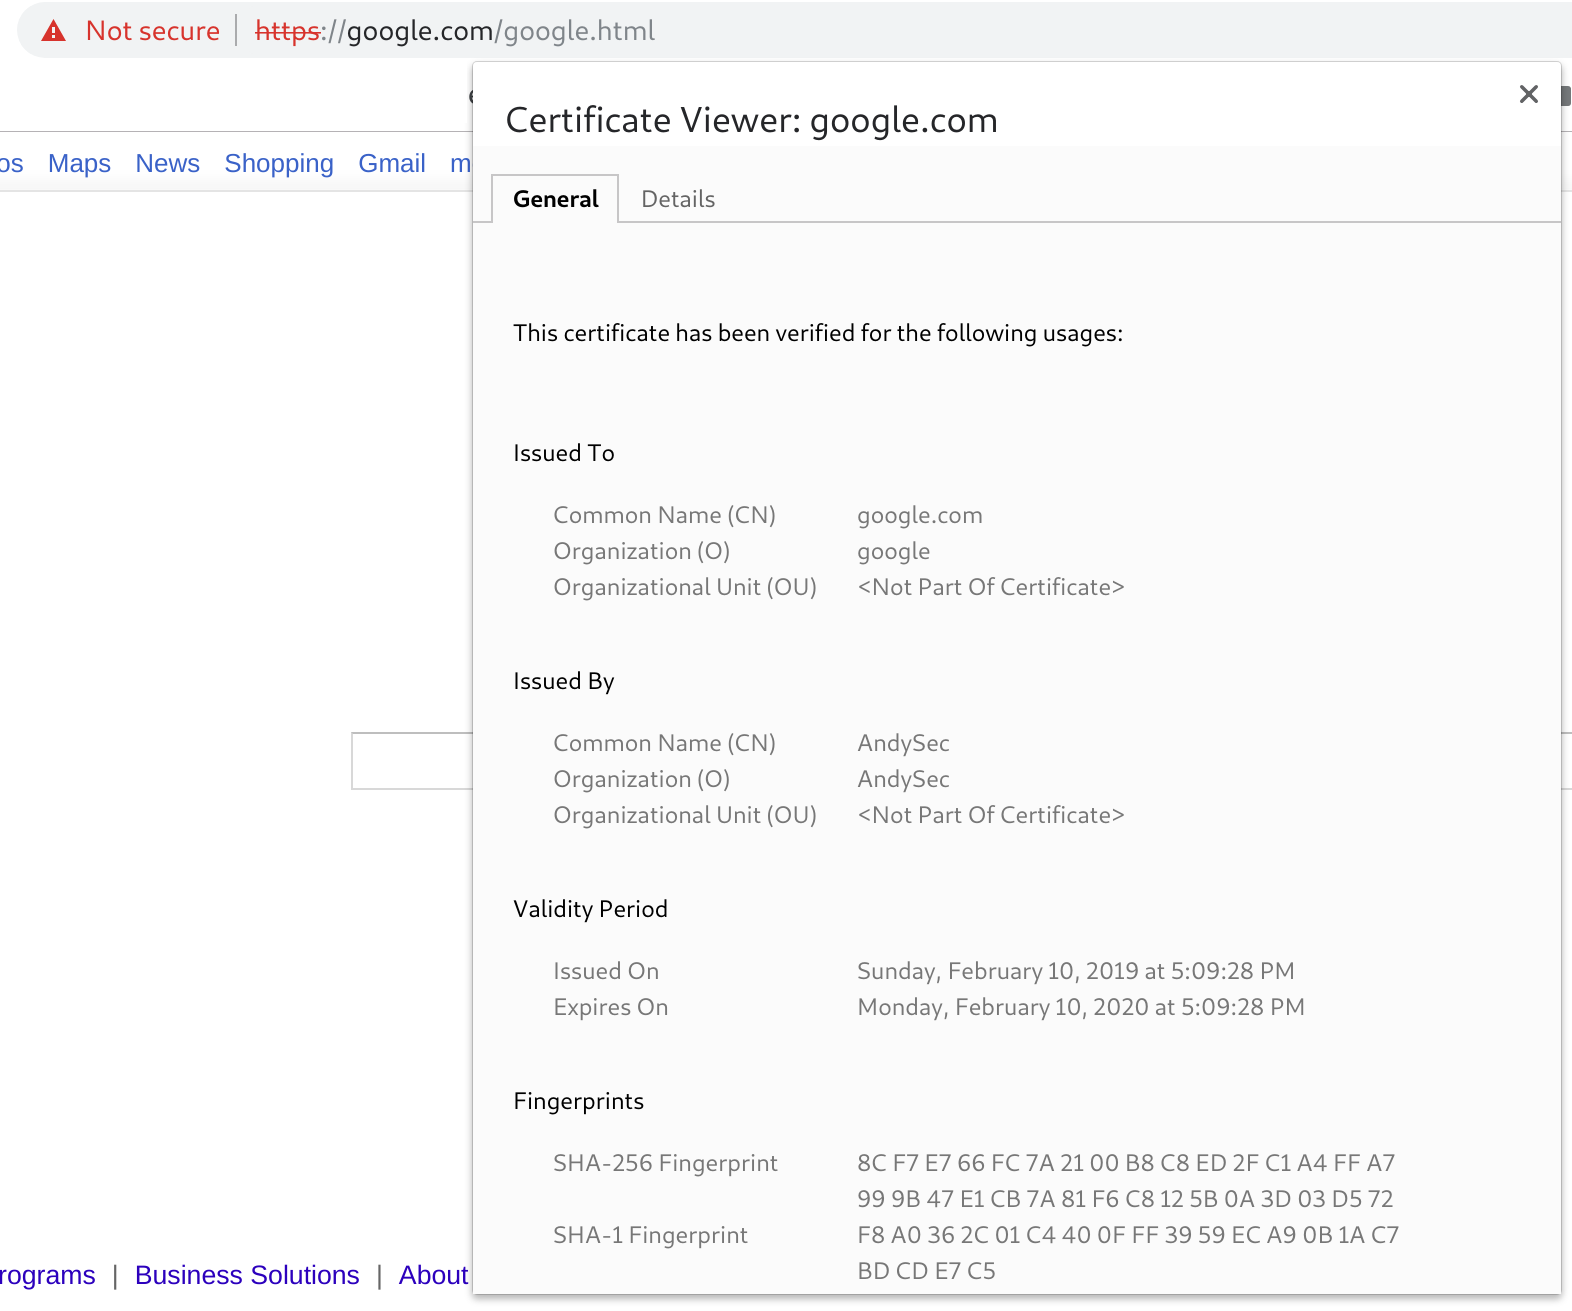
\includegraphics[width=\textwidth]{chrome.png}
\end{figure}

After you imported the CA to the trustful CAs. You don't get any warning and a green locked key lock sign, as you can see in figure \ref{fig:firefox}. So for the first view anybody can't see any difference compared to the original site except that the faked one is out of date.. 
Only if you click to see the details you see the same detailed informations about it as in chrome respectively decribed before.


\begin{figure}[htp]
    \centering
    \caption{Screenshot of Firefox}
    \label{fig:firefox}
    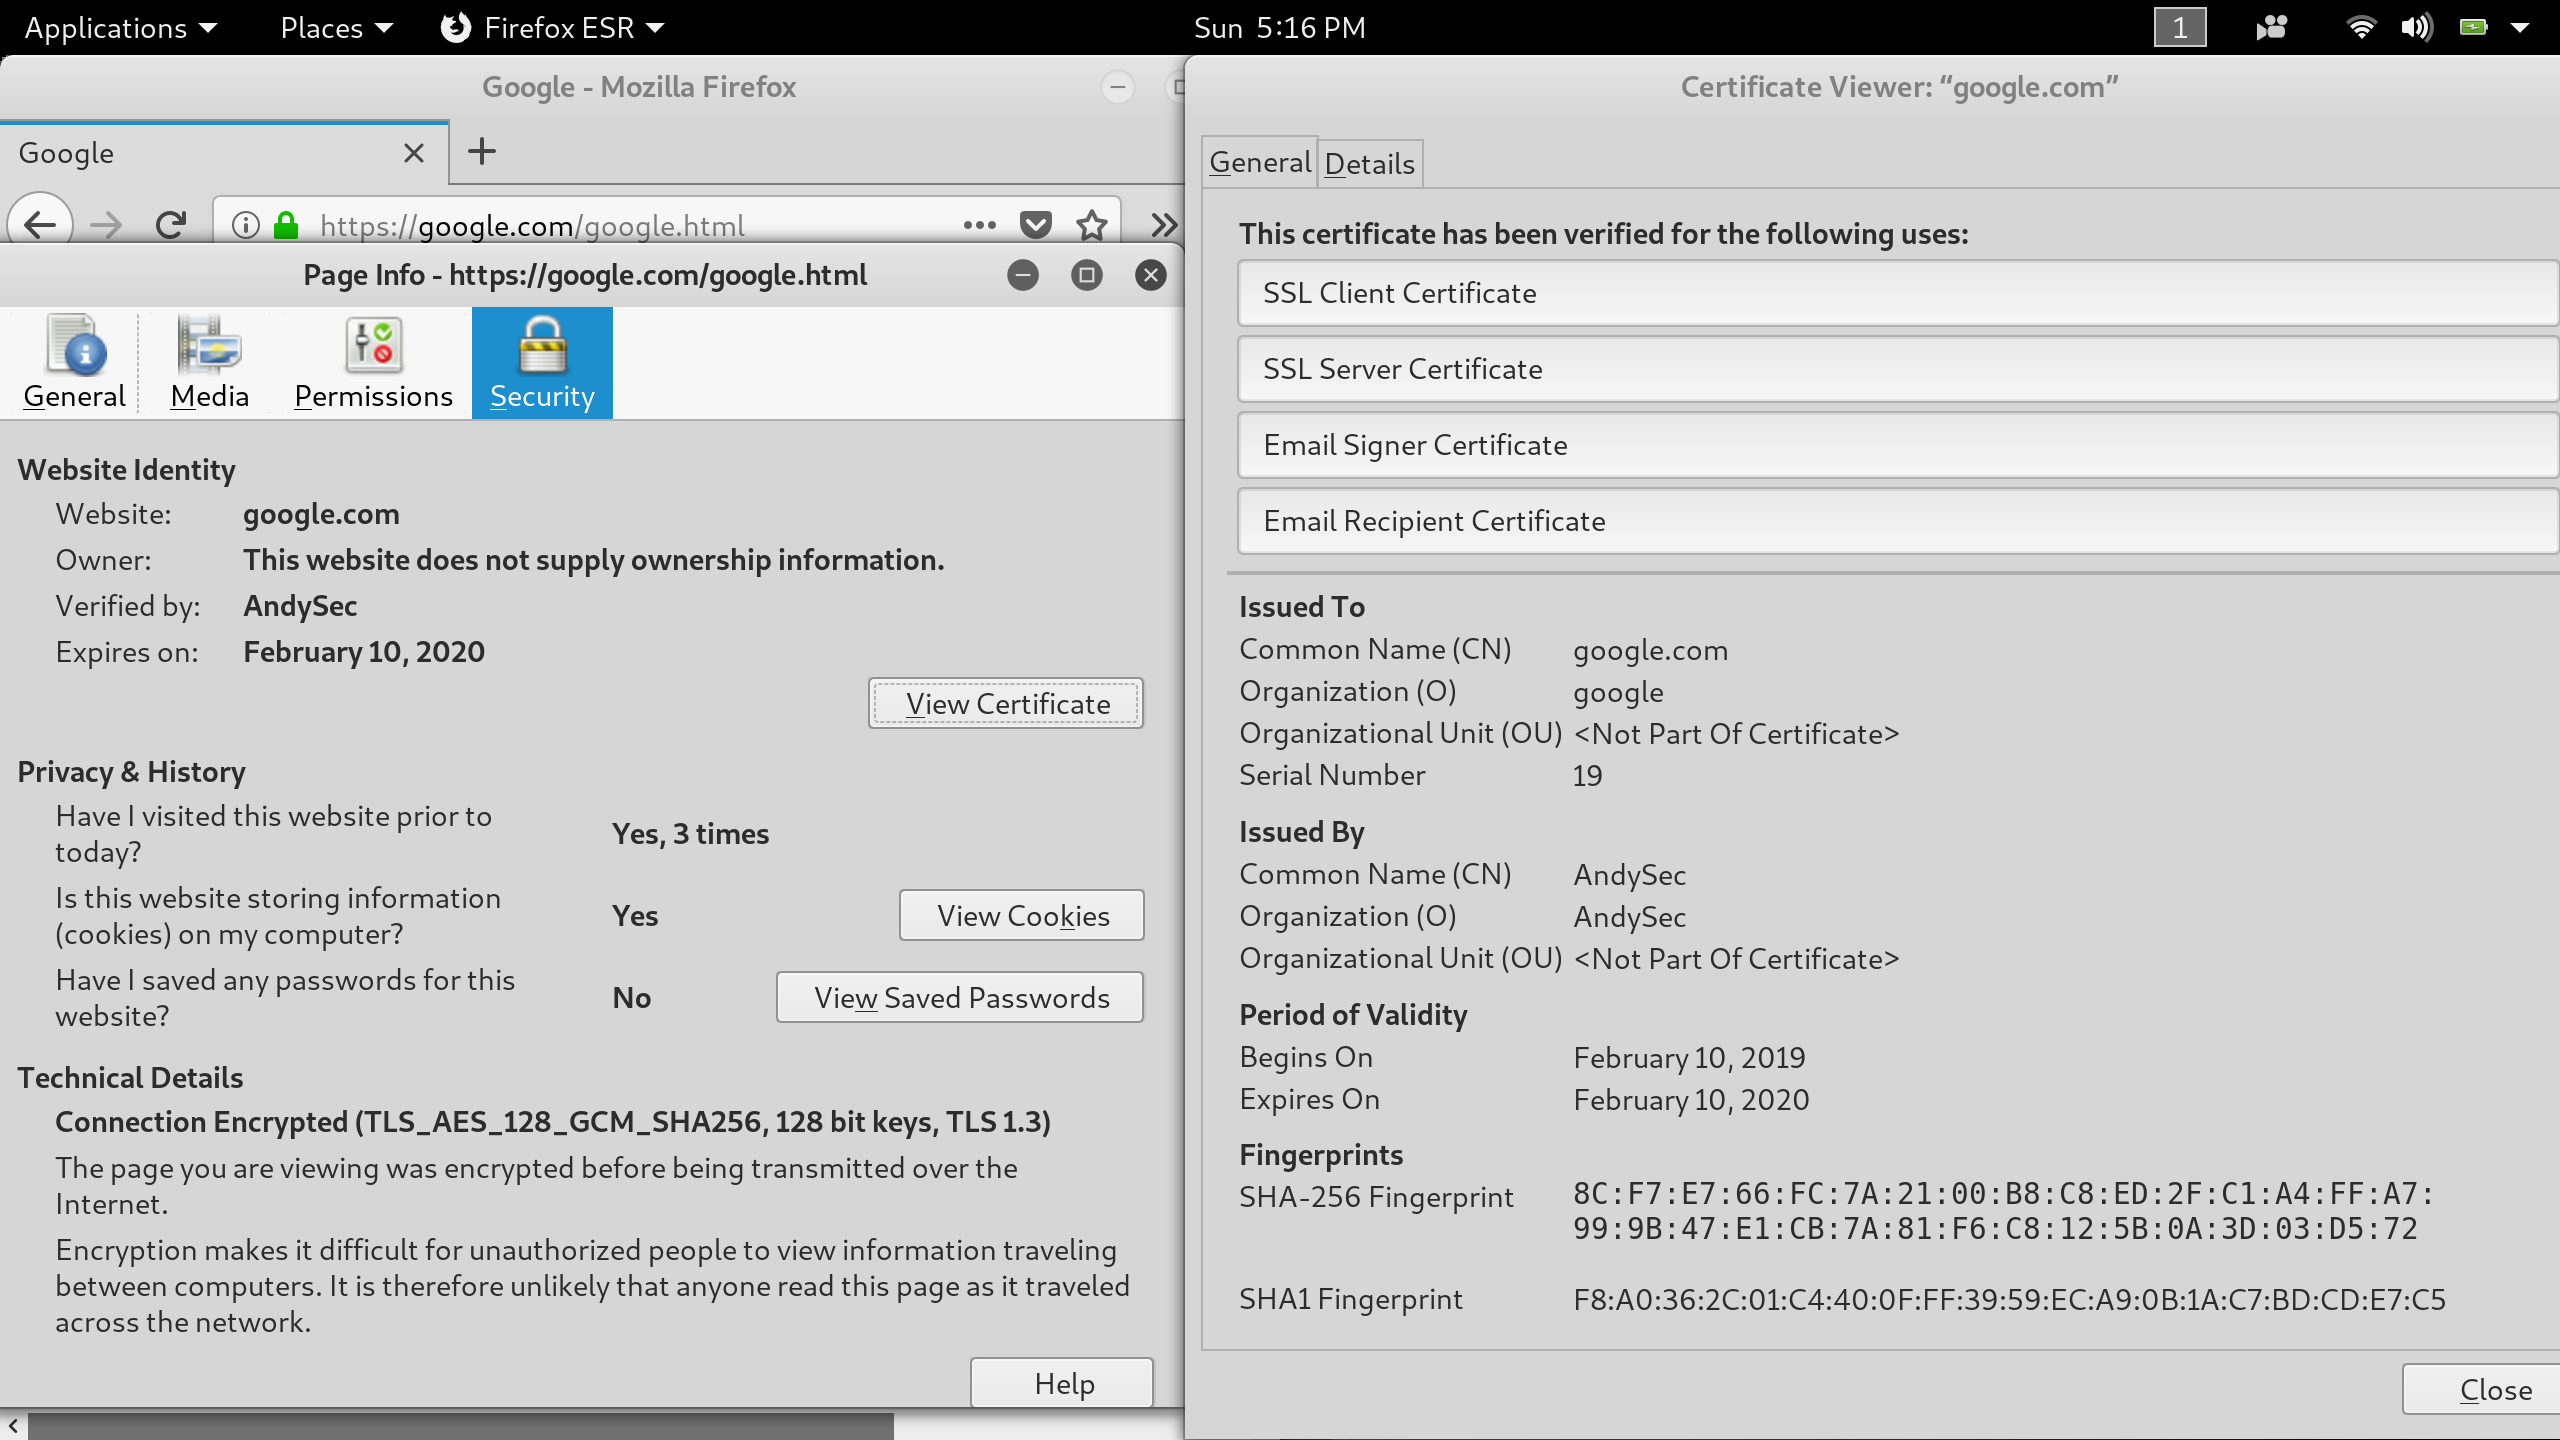
\includegraphics[width=\textwidth]{firefox.png}
\end{figure}


\section{Password Files}

\textit{What do you observe?}\\
Well, for doing this, you obviously need superuser rights. When you open it as superuser you also only see the hash.\\

\textit{What is the hash of your password? What is the date of your last password change?}\\
I won't publish my password, neiter the hash, sry!
The number in the shadow file is 17908. This means 17908 days after January 1st 1970. So the actual date is January 12th 2019. That's the date where I set up the system.\\

\textit{What algorithm was used to protect your password? What is the value of the salt used to protect your password?}\\
The SHA-512 algorithm was used to protect the password. The salt is \textit{jn2qldDW}. The characters in \textit{salt} are drawn from the set [a-zA-Z0-9./]. The encrypted password string contains 86 characters.\\


\section{Password Cracking}
\lstinputlisting[caption=Code of task 4, label=lst:task4]{task4.py}

\subsection{A}

\textit{By just looking at the hashes, what can you learn about an individual user’s passwords? Is there anything you can learn about the passwords of all the users from this password file?}\\
The passwords has all the same encryption. Furthermore all user are using a different password. They are encrypted using SHA-1 and bas64-encoded.


\subsection{B}

\textit{If your program completes (i.e. hashes all the words in the dictionary) without finding a match, what can you assume about the passwords? Which passwords were you able to crack?}\\
If the program would complete without finding a match, the passwords would be well choosen, at least they contain no usual words which are in such simple dictionaries. However it could also be words in different languages, which are not in this special dictionary.\\
The user \textit{zachary} used the password \textit{awesome}.\\


\subsection{C}

\textit{Which additional passwords did you crack?}\\
User \textit{ellie} has used PW: \textit{2cute4u}\\
User \textit{jamie} has used PW: \textit{password1}\\
User \textit{newton} has used PW: \textit{zaq12wsx}\\

\textit{Were you able to crack all the passwords? Why or why not? If not, what characteristics do you think the un-cracked password has?}\\
I wasn't able to crack the passwords of \textit{copernicus} and \textit{clara}. The passwords could be some real random ones, at least not any with simple combinations which are listed in this dictionary.\\


\textit{For those passwords you were unable to crack, what would be required to crack them and how do you think it would take?}\\
You could for example brute-force them including the birthday attack. You would need 2\textsuperscript{80} SHA-1 evaluations, which will take long. With more efficient methods you would still need about 2\textsuperscript{60} evaluations which is in result 6,500 years of single-CPU computations and 110 years of single-GPU computations. But nowadays with renting stacks of GPUs, the needed time gets really small.\\


\textit{Using each of the cracked passwords, go to the user's respective web page. What is the secret word for each user?}\\
For user \textit{zachary} the secret word is 'This is my world now.'\\
For user \textit{ellie} the secret word is 'Hoochie Mama!'\\
For user \textit{jamie} the secret word is 'I've made a huge mistake.'\\
For user \textit{newton} the secret word is 'S'up dawg.'\\
